\documentclass[a4paper,12pt]{article}
\usepackage[utf8]{inputenc}
\usepackage{graphicx}
\usepackage{float}
\usepackage[spanish]{babel}
\usepackage{listings}

%opening
\title{Tarea No. 15. Patrón Front Controller y CDI}
\author{Barrera Pérez Carlos Tonatihu \\ Profesor: José Asunción Enríquez 
Zárate \\ Web Application Development \\ Grupo: 3CM9 }

\begin{document}

\maketitle
\newpage

\section{Desarrollo}
El patrón de diseño front controller significa que todas las peticiones que 
vienen por un recurso en una aplicación serán manejadas por un solo manejador y 
después serán enviadas al respectivo manejador dependiendo del tipo de 
solicitud. El front controller puede usar auxiliares para lograr el mecanismo 
de envío.
uml-front-controller-design-pattern

\begin{figure}[H]
    \begin{center}
    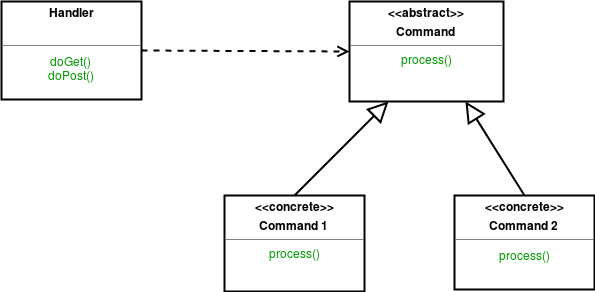
\includegraphics[width=\textwidth]{uml-front-controller-design-pattern.png}
    % estructura.png: 800x436 px, 96dpi, 21.16x11.53 cm, bb=0 0 600 327
    \caption{Patrón Front Controller}
    \label{fig:diagrama}
    \end{center}
\end{figure}


\begin{itemize}
 \item [Controlador]. El controlador es el punto de contacto inicial para el 
manejo de las peticiones en el sistema. El controlador delega a un auxiliar 
para completar la autenticación y autorización de un usuario o para inicializar 
la recuperación de contactos.
\item [Vista]. Una vista representa y despliega información al cliente. La 
vista recupera información del modelo. Los auxiliares apoyan a las vistas 
mediante el encapsulado y adaptación del subyacente modelo de datos para su uso 
en la visualización.
\item [Despachador]. Es el responsable del manejo de las vistas y la 
navegación, manejando la elección de la siguiente vista a presentar al usuario, 
y proveyendo el mecanismo para el control de vectores de este recurso.
\item [Auxiliar]. Es el responsable de ayudar a la vista o el controlador a 
completar su proceso. Así, los auxiliares tienen numerosas responsabilidades, 
incluyendo el recolectado de datos requeridos por la vista y ordenando este 
modelo intermedio, en cuyo caso el auxiliar es algunas veces referido como un 
bean de valor. 
\end{itemize}

\subsection{Ventajas y desventajas}
Las ventajas que presenta este patrón son las siguientes:
\begin{itemize}
 \item [Control centralizado]. Este patrón maneja todas las peticiones a la 
aplicación. Esta implementación centralizada del control evita el uso de 
múltiples controladores, es deseable para hacer cumplir políticas de toda la 
aplicación, como el seguimiento y la seguridad de los usuarios.
\item [Seguridad de hilos]. Un nuevo objeto de mando surge cada que se recibe 
una solicitud y estos objetos no están diseñados para ser seguros para 
subprocesos. Por lo tanto, sera seguro en las clases de mando. Aunque la 
seguridad no está garantizada cuando se reúnen los problemas de subprocesos, 
los códigos que actúan con el mando aun son seguros para subprocesos.
\end{itemize}

Sin embargo, se presentan las siguientes desventajas:
\begin{itemize}
 \item No es posible escalar la aplicación utilizando este patrón.
 \item El desempeño es mejor si se lidia solo con una única petición.
\end{itemize}
\section{Conclusiones}

\end{document}
